%-------------------------------------------------------------------------------
\section{Introduction}
%-------------------------------------------------------------------------------
Web application developers today have more incentives than ever to provide better privacy for their
users.
%
Laws like the EU's General Data Protection Regulation (GDPR)~\cite{eu:gdpr} and California's
Consumer Privacy Act (CCPA)~\cite{ca:privacy-act} codify users' rights and associate legal
consequences and reputational damage with data breaches~\cite{breach:amazon,
breach:twitter, breach:fb, breach:marriott, breach:quora}.
%
Beyond legal mandates, it is good practice to minimize user data retained.
%

%
Consequently, application developers increasingly face the need to implement implement
\emph{privacy transformations} over their applications' data.
%
For example, GDPR compliance requires a transformation that deletes a user's account and
data, and anonymizes any data retained due to legal requirements or to preserve
application utility for other users.
%
As another example, consider the possibility of anonymizing old peer review data in a 
system like HotCRP~\cite{hotcrp}, to avoid having a future data breach expose reviewer
identities.
%
Today, developers must manually implement these transformations as part of their application
code, which is error-prone, laborious, and begets ad-hoc solutions.
%

%
%To write a privacy transformation, developers must carefully map the high-level privacy policy to
%operations that delete or rewrite data objects, while ensuring that the application preserves
%utility for other users, retains legally-mandated anonymized data, and avoids violating application
%invariants.
%
%For example, deleting a user's account should not unexpectedly grant broad access to
%previously-private content by deleting objects that restrict access, nor should it make
%non-sensitive shared content disappear.
%%
%Developers must also consider indirectly identifying correlations between data objects: for example,
%anonymized public running routes can identify the user's hometown and even the
%user~\cite{strava:heatmap}, and anonymized order histories in e-commerce sites can reidentify
%buyers.

\begin{figure}[t]
    \centering
    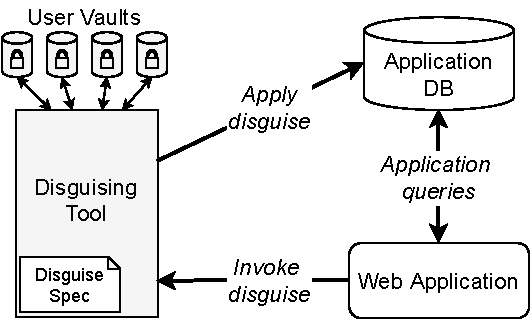
\includegraphics[width=0.35\textwidth]{img/disguise_tool}
    \caption{A data disguising tool takes a developer's disguise specification and transforms
	     a web application's database contents. Per-user vaults
	     (which can be encrypted and stored on third-party storage) support reversible
	     privacy transformations by logging the changes to each user's data.}
    \label{fig:tool}
\end{figure}

%
%The burden of implementing privacy transformations grows with the underlying privacy policy's
%complexity.
%
%Although simplicity has advantages, more nuanced privacy policies are important and useful.
%
%Such policies can help protect users against data correlation attacks; they can give more
%control to individuals by allowing them to choose their own, fine-grained privacy semantics; and
%they may enable new privacy modes such as data that gradually ``decays'' to become less identifiable over time.
%
%Likewise, reversible privacy transformations might strike a sweet
%spot---allowing users to remove identifiable information on demand,
%but accommodating service providers' interest to make it easy for users to return---but
%add significant implementation burden.
%

%
%With more nuanced and reversible privacy transformations, developers face an even greater challenge:
%they must reason about how these privacy transformations compose. For example, an application may
%automatically decay data over time, but must still correctly remove a user's data when they delete
%their account, even if this data has been anonymized.
%Ensuring that one privacy transformation does not affect the privacy properties
%achieved by future transformations, even if they both transform the same data, is a non-trivial task.
%

%
In this paper, we propose \emph{data disguising}, a new systematic framework that helps developers
of database-backed web applications specify, implement, and reason about privacy transformations.
%
Data disguising supports a broad range of privacy transformations and separates the application
of privacy transformations (``data disguises'') from application code.
%
Developers provide a disguise specification to an external tool, which computes the necessary
database changes and applies them to the application's database backend (Figure~\ref{fig:tool}).
%
Applying a disguise transforms the state of application data in privacy-preserving ways (\eg
deleting users' identifiers, or decorrelating identifying object relationships) while preserving
application invariants and utility.
%
Since many data disguises edit the physical database contents in (often necessarily)
information-destroying ways, the disguising framework includes \emph{per-user vaults}.
These vaults are individually owned storage shards that log all disguises applied to a single user's data,
and cannot be accessed by application's queries.
%
If a disguise should be reversed, either through explicit action---\eg a user might choose to return
to the application---or in order to apply a second, data-dependent
disguise---the disguising tool accesses the relevant user vaults to obtain the original,
unmodified data.
\lyt{The implicit reversal for data-dependent disguises is confusing, need to edit this.}
%
Vaults can be deployed in different ways and for different levels of privacy guarantee: they
might be physically co-located or separate from the the application storage, encrypted or
unencrypted, and access might require explicit user approval.
%

%
We believe that flexible disguising is what real applications require, and that better user
privacy on the web is best achieved through a systematic approach that reduces developer
burden.
%
However, our framework is far from complete and realizing it will require solving several
research problems.
%
First, when an application contains more than one privacy transformation, the respective
data disguises may have co-dependencies: for example, removing a user's data on account
deletion is challenging if that data has already been anonymized and decorrelated from the
user, and not all disguises may be reversible.
%
A practical data disguising tool could use a combination of static analysis, warnings to
developers, and privacy assertions to ensure disguises compose correctly.
%
Second, the performance impact of data disguises could be substantial, particularly if they
transform many database rows, particularly if applied on a live application database.
%
We argue that these are important challenges for researchers to investigate to make data
disguising practical.
%
Our proof-of-concept data disguising tool, \sys, demonstrates the potential of this
approach.
%
%Disguises do not guarantee strict privacy---a disguise's content might still expose user
%information or correlated data if not redacted by the policy---but flexible disguising,
%rather than universal deletion, is what real applications require.
%
%Disguises consist of transformations performed on the high-level object graph embedded in
%database-based applications (encoded by \eg foreign key relationships in relational
%databases)~\cite{orms}.
%
%A data disguising tool takes a disguise and its target, and automatically applies the appropriate
%transformations to application data to achieve the disguised state, handling
%disguise composition and disguise interdependencies. Developers can
%thus reason at a high level about each disguise in isolation, reducing the developer burden.
%
%
%\sys proxies relational database operations and exposes APIs to invoke privacy transformations.
%
